\documentclass[14pt]{article}

\usepackage[utf8x]{inputenc}
\usepackage[russian]{babel}
\usepackage{graphicx}
\usepackage{caption}
\usepackage{float}
\graphicspath{{images/}}
\DeclareGraphicsExtensions{.pdf,.png,.jpg}

\usepackage{amsmath}
\usepackage{pgfplots}

\usepackage{geometry} % Меняем поля страницы
\geometry{left=2cm}% левое поле
\geometry{right=1.5cm}% правое поле
\geometry{top=2cm}% верхнее поле
\geometry{bottom=2cm}% нижнее поле

\renewcommand{\theenumi}{\arabic{enumi}}
\renewcommand{\labelenumi}{\arabic{enumi}}
\renewcommand{\theenumii}{.\arabic{enumii}}
\renewcommand{\labelenumii}{\arabic{enumi}.\arabic{enumii}.}
\renewcommand{\theenumiii}{.\arabic{enumiii}}
\renewcommand{\labelenumiii}{\arabic{enumi}.\arabic{enumii}.\arabic{enumiii}.}

\begin{document}
\begin{titlepage}
	\begin{center}
		\fontsize{18pt}{20pt}\selectfont
		\textbf{Работа 4.4.4}
	
		\vspace{5cm}
		\fontsize{24pt}{25pt}\selectfont
		Интерферометр Фабри-Перо
	\end{center}
	\begin{flushright}
		\fontsize{18pt}{20pt}\selectfont
		\vspace{14cm}
		\hspace{-3cm}
		\textit{Корнеев Е.С.}
	\end{flushright}		
\end{titlepage}

\begin{center}
	\fontsize{16pt}{18pt}\selectfont	
	Интерферометр Фабри-Перо
\end{center}


\fontsize{14pt}{16pt}\selectfont
\vspace{1cm}
\textbf{Цель работы:} Изучение интерферометра Фабри-Перо и определение
его характеристик, как спектрального прибора.

\vspace{0.5cm}
\textbf{Оборудование:} интерферометры Фабри-Перо, линзы, светофильтр,
ртутная лампа ПРК-2, высокочастотная натриевая лампа,
катетометры КМ-6. 

\vspace{0.5cm}
Интерферометр Фабри-Перо как спектральный прибор высокой разрешающей
силы находит широкое применение в лабораторной практике.
Он предназначен главным образом для исследования тонкой структуры
спектральных линий, а также является неотъемлемым элементом любого
лазера, где выполняет роль оптического резонатора.

\begin{figure}[H]
	\center{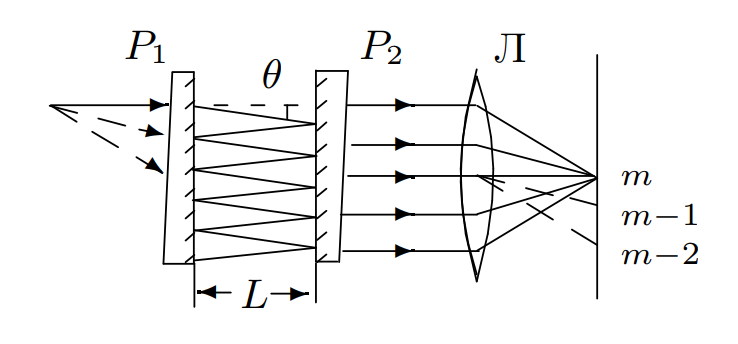
\includegraphics[width = 11cm]{1}}
	\caption{Интерферометр Фабри-Перо}
	\label{fig:image}
\end{figure}

Интерферометр Фабри-Перо состоит из двух стеклянных (или кварцевых)
пластин $P_1$ и $P_2$ (рис. 1), внутренние плоские поверхности которых
хорошо отполированы (с точностью до $10^{-2}\lambda$) и установлены параллельно
друг другу. На эти поверхности наносятся хорошо отражающие покрытия.
Наряду с металлическими покрытиями (Ag, Al), для которых
коэффициент отражения $r \approx 0.9$, в настоящее время широко применяются
диэлектрические многослойные интерференционные покрытия, для
которых $r \approx 0.99$ и даже выше. Наружные поверхности пластин обычно
составляют небольшой угол с внутренними, чтобы световой блик, отраженный
от наружных поверхностей, не мешал наблюдениям.

Интерферометр Фабри-Перо можно рассматривать как плоскопараллельную
воздушную пластину, на которой происходят многократные
отражения и интерференция световых лучей. Интерференционная
картина, наблюдаемая в фокальной плоскости линзы Л, состоит из концентрических
колец равного наклона. Для двух соседних лучей, распространяющихся
между зеркалами интерферометра под углом $\theta$, разность
хода определяется соотношением
\begin{equation}
	\Delta = 2L\cos\theta
\end{equation}

\noindent где $L$ -- расстояние между зеркалами интерферометра. Равенство (1) —
частный случай известной формулы для плоскопараллельной пластины с показателем преломления
$n: \Delta = 2Ln\cos\psi; \psi$ -- угол преломления луча в пластине.

Пусть $r$ и $t$ -- коэффициенты отражения и пропускания зеркал интерферометра
(по интенсивности). Если амплитуду падающей волны обозначить через
$A_0$, то амплитуда первого луча, прошедшего через интерферометр, равна
$A_0t$, второго $A_0tr$, третьего $A_0tr^2$ и т.д. В комплексном
представлении амплитуды этих лучей составляют бесконечную геометрическую
прогрессию
\begin{equation}
	A_0t,~A_0tre^{ik\Delta},~A_0tr^2e^{2ik\Delta},~A_0tr^3e^{3ik\Delta}, ...
\end{equation}

\noindent где $k = 2\pi/\lambda$ -- волновое число для света. Знаменатель прогрессии равен
$re^{ik\Delta}$. В фокальной плоскости линзы происходит сложение всех лучей.
Результирующая амплитуда равна
\begin{equation}
	A = \frac{A_0t}{1 - re^{ik\Delta}}
\end{equation}

\noindent Найдем интенсивность $I$ прошедшего света:
\begin{equation}
	I = AA* = \frac{I_0t^2}{1 + r^2 - 2r\cos(k\Delta)}
\end{equation}

\noindent где $I_0 = A^2_0$ -- интенсивность падающей волны. На рис. 2 представлена
зависимость отношения $I/I_0$ от порядка интерференции $\Delta/\lambda$ для разных
значений коэффициента отражения. Как видно из (4), максимумы этого распределения достигаются
при целых значениях $\Delta/\lambda$. При этом $I_{max} = I_0$, т. е. интерферометр в этом случае
является идеально прозрачной системой. Разумеется, этот результат справедлив только в отсутствие
поглощения света в зеркалах.

При достаточно больших значениях коэффициента отражения $(r \geq 0,9)$ интерференционная
картина состоит из узких светлых колец, разделенных широкими темными промежутками. Это является следствием
интерференции большого числа лучей (многолучевая интерференция). При $r \leq 0,1$ наблюдается плавное чередование
слабо выраженных максимумов и минимумов, характерное для интерференции двух лучей, сильно
различающихся по амплитуде.

\vspace{0.5cm}
\textbf{Измерение длин волн $\lambda$ и расстояний $d\lambda$ между спектральными линиями.}
Исследуем диаметры интерференционных колец, предполагая для простоты, что углы $\theta$ достаточно малы.
Рассмотрим два интерференционных кольца, для которых порядки интерференции $\Delta/\lambda$ равны
$m_i$ и $m_j$ . Из формул (1) и (4) следует, что светлое кольцо порядка $m$ образуется при
\begin{equation}
	\Delta = 2L\cos\theta = m\lambda,~~m \in Z
\end{equation}

\begin{figure}[H]
	\center{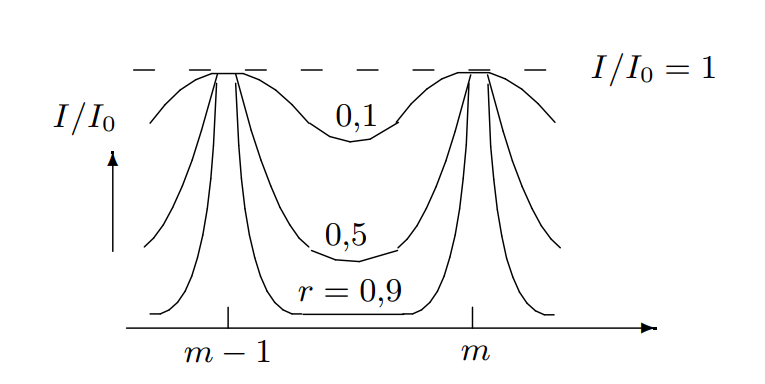
\includegraphics[width = 11cm]{2}}
	\caption{Распределение интенсивности в проходящем свете в зависимости от порядка интерференции $\Delta/\lambda$}
	\label{fig:image}
\end{figure}

\noindent Отметим, что порядок интерференции возрастает при переходе к кольцам меньшего диаметра, т.е.
при уменьшении угла $\theta$.

При малых $\theta$ имеем
\begin{equation}
	2L\left(1 - \frac{\theta_i^2}{2}\right) = m_i\lambda;~~2L\left(1 - \frac{\theta_l^2}{2}\right) = m_j\lambda
\end{equation}

\noindent Вычитая второе уравнение из первого и принимая во внимание, что при
переходе к соседнему кольцу порядок интерференции меняется на единицу, получим
$$
	L(\theta_j^2 - \theta_i^2) = (m_i - m_j)\lambda = (j - i)\lambda
$$

\noindent В приведенной формуле номера колец $i$ и $j$ отсчитываются от центра.

Диаметр $D$ кольца в фокальной плоскости линзы Л связан с её фокусным расстоянием
$f$ соотношением
\begin{equation}
	D = 2f\theta
\end{equation}

\noindent Следовательно,
\begin{equation}
	\lambda = \frac{L}{4f^2}\frac{D_j^2 - D_i^2}{j - i}
\end{equation}

\noindent Эта формула используется при измерении длины волны света с помощью
интерферометра Фабри-Перо или для определения постоянной интерферометра
$L$ по известному значению $\lambda$.

Пусть теперь в интерферометре Фабри-Перо наблюдается система колец для двух близких спектральных линий
$\lambda$  и $\lambda + d\lambda$. Дифференцируя (5), при малых $\theta$ найдем
$$
	-2L\theta d\theta = md\lambda
$$

\noindent откуда следует:
\begin{equation}
	d\lambda = -\frac{2L\theta}{m}d\theta \approx -\lambda\theta d\theta = -\frac{\lambda \overline{D}}{4f^2}dD
\end{equation}

\noindent где $\overline{D}$ -- средний диаметр колец, a $dD$ -- разность диаметров колец,
образующихся для спектральных линий с длинами волн $\lambda$ и $\lambda + d\lambda$ при
одинаковом порядке интерференции. С помощью формулы (9) можно определять $d\lambda$, не зная постоянной
интерферометра $L$.

Выбирая прибор для исследования спектра, обычно сравнивают три характеристики: \textsl{дисперсию}, \textsl{дисперсионную область} и
\textsl{разрешающую способность}.

\vspace{0.5cm}
\textbf{Дисперсия интерферометра.} Отношение расстояния $dl$ между спектральными линиями в плоскости спектра
к разности длин волн $d\lambda$ этих линий называют \textsl{линейной дисперсией} $D^*$ спектрального прибора $(D^* = dl/d\lambda)$
и выражают обычно в миллиметрах на ангстрем. Можно выразить линейную дисперсию $D^*$ через угловую $(d\theta/d\lambda)$. Как следует из
формулы (9), для интерферометра Фабри-Перо
$$
	D^* = f\frac{d\theta}{d\lambda} = \frac{dD}{2d\lambda} = \frac{2f^2}{\lambda D}
$$

\noindent Высокая дисперсия является основным преимуществом интерферометра Фабри-Перо.

\vspace{0.5cm}
\textbf{Дисперсионная область.} Областью дисперсии спектрального прибора называют максимальный интервал длин волн
$\Delta\lambda$, при котором еще не происходит перекрытия интерференционных полос соседних порядков.
Ширина этой области определяется изусловия наложения кольца $(m + 1)$-го порядка для длины волны
$\lambda$ и кольца $m$-го порядка для длины волны $\lambda + \Delta\lambda$:
$$
	m(\lambda + \Delta\lambda) = (m + 1)\lambda
$$
\noindent откуда
\begin{equation}
	\Delta\lambda = \frac{\lambda}{m} \approx \frac{\lambda^2}{2L}
\end{equation}

\noindent Порядок интерференции $m$ в интерферометрах Фабри-Перо чрезвычайно высок. Так, для $\lambda = 5\cdot10^{-5}$ см и
$L = 0,5$ см получаем: $m \approx 2L/\lambda = 2\cdot10^4$. Область дисперсии при этом равна $\Delta\lambda = 0,25$\r{A}.
Таким образом, спектральный интервал, который можно анализировать с помощью интерферометра Фабри-Перо, весьма мал.
Поэтому перед интерферометром Фабри-Перо обычно располагают светофильтр или другой спектральный прибор, вырезающий
спектральную полосу, не превышающую $\Delta\lambda$. Отметим, что если спектральная полоса $\Delta\lambda$ исследуемого
излучения известна, то с помощью формулы (10) можно определить допустимое значение постоянной интерферометра $L$.

\vspace{0.5cm}
\textbf{Разрешающая способность интерферометра Фабри–Перо.} Разрешающая способность спектрального прибора определяетя
отношением
\begin{equation}
	R = \frac{\lambda}{\delta\lambda}
\end{equation}

\noindent где $\delta\lambda$ -- минимальная разность длин волн, разрешимая прибором вблизи длины волны $\lambda$.
При определении $\delta\lambda$ обычно используют условный критерий разрешения Релея, согласно которому две линии разрешаются,
если их максимумы отстоят друг от друга на половину их ширины. Определяя ширину линии на уровне, на котором интенсивность падает
в два раза по сравнению с максимальным значением в середине линии, можно получить из (4):
\begin{equation}
	R \approx \frac{2\pi L\sqrt{r}}{\lambda(1 - r)}
\end{equation}

\noindent Мы приведем здесь другой вывод формулы (12), в котором интерферометр Фабри-Перо рассматривается
как оптический резонатор, аналогичный любой колебательной системе, например, колебательному контуру в
радиотехнике. Эта аналогия опирается на сходство формы линии интерферометра (рис. 2) с резонансной кривой. Обратим внимание также на
то, что определение добротности $Q$ колебательной системы аналогично определению разрешающей способности $R$ спектрального прибора в оптике:
$$
	Q = \frac{\omega}{\delta\omega},~~~R = \frac{\lambda}{|\delta\lambda|} = \frac{\omega}{|\delta\omega|}
$$

\noindent Но, как известно,
\begin{equation}
	Q = 2\pi\frac{W}{\Delta W_T}
\end{equation}

\noindent где $W$ -- запас энергии колебательной системы, $\Delta W_T$ -- потеря энергии за период колебаний. Найдем величину
$Q$ для интерферометра Фабри-Перо, рассматривая его как оптический резонатор. Для этого рассмотрим рассеяние оптической энергии в
возбужденном резонаторе.

Пусть в некоторый момент времени между зеркалами интерферометра локализована оптическая энергия $W$. Излучение внутри интерферометра
имеет характер двух бегущих в противоположных направлениях волн. Вследствие конечной прозрачности зеркал энергия каждой волны за время
$\tau = L/c$ пробега между зеркалами ослабится в $(1 - r)$ раз. Следовательно,
$$
	\Delta W_T = (1 - r)W
$$

\noindent Нас интересуют потери за период $T = \lambda/c$:
$$
	\Delta W_T = \frac{T}{\tau}\Delta W_\tau = \frac{\lambda(1 - r)}{L}W
$$

\noindent Подставляя это значение в формулу (13), найдем
\begin{equation}
	Q \approx \frac{2\pi L}{\lambda(1 - r)}
\end{equation}

\noindent что для хороших зеркал $(r \approx 1)$ совпадает с (12) с точностью до несущественного
множителя $\sqrt{r}$.

Из формул (12) и (14) следует, что при $r \rightarrow 1$ добротность $Q \approx R \rightarrow \infty$.
Однако на самом деле этого не проис ходит. При $r$, достаточно близких к единице, существенное влияние на разрешающую
способность начинает оказывать рассеяние света из-за неоднородностей поверхностей зеркал. Например, при $r \approx 95\%$ глубина
неровностей поверхности должна быть меньше $\lambda/50$.

\vspace{0.5cm}
\textbf{Экспериментальная установка.} Схема установки для изучения работы интерферометра Фабри-Перо представлена на рис. 3.
Свет от ртутной лампы $S$, пройдя через линзу Л$_0$ и зелёный светофильтр С, попадает в интерферометр Фабри-Перо (ИФП). Линза
Л$_0$ служит для формирования пучка лучей (слегка сходящегося или слегка расходящегося). Интерференционные кольца наблюдаются в
фокальной плоскости линзы Л. Картина рассматривается через зрительную трубу Т, сфокусированную на эту плоскость. Диаметры колец
измеряются с помощью отсчётного микроскопа (не показанного на рис. 3).

\begin{figure}[H]
	\center{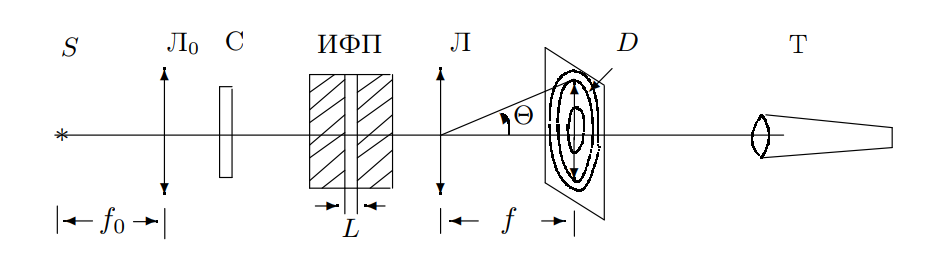
\includegraphics[width = 15cm]{3}}
	\caption{Схема экспериментальной установки}
	\label{fig:image}
\end{figure}

Зрительная труба Т и отсчётный микроскоп -- это составные части катетометра -- прибора, предназначенного для измерения расстояний
в вертикальной плоскости.

При достаточной яркости ртутной лампы можно увидеть, что зелёная линия ртути состоит из нескольких компонентов. Расщепление этой
спектральной линии связано с дополнительной энергией, возникающей как в результате взаимодействия магнитных моментов ядра и электрона
-- сверхтонкая структура (магнитное поле ядра действует на спиновый магнитный момент электрона), так и с изотопическим сдвигом
(в парах ртути присутствуют в заметных количествах изотопы с атомными массами от 198 до 204 а.е.м.). Каждое зелёное кольцо содержит
более десятка близко расположенных компонент, но разрешение нашего прибора не позволяет все их рассмотреть. Спектр натриевой лампы
исследуется по аналогичной схеме, но светофильтр в этом случае не нужен, а интерферометр, линзы и зрительная труба катетометра имеют
другие параметры.

\vspace{2cm}
\textbf{Ход работы.}

Снимем координаты нижней и верхней части кольца, чтобы определить диаметр колец:

\begin{center}
\begin{tabular}{|c|c|c|c|c|c|c|c|c|c|c|c|}
\hline
$N$	&	$x_\text{низ }$, мм		&	$x_\text{верх}$, мм		&	$D$, мм		&	$D^2$, мм$^2$	\\
\hline
7'	&	145.363					&	186.039					&	40.676		&	1654			\\
\hline
7	&	145.793					&	185.588					&	39.759		&	1583			\\
\hline
6'	&	146.630					&	184.747					&	38.117		&	1457			\\
\hline
6	&	147.225					&	184.260					&	37.035		&	1371			\\
\hline
5'	&	148.210					&	183.005					&	34.795		&	1210			\\
\hline
5	&	148.843					&	182.610					&	33.767		&	1140			\\
\hline
4'	&	149.983					&	181.437					&	31.454		&	989 			\\
\hline
4	&	150.576					&	180.705					&	30.129		&	907 			\\
\hline
3'	&	151.955					&	179.407					&	27.452		&	753 			\\
\hline
3	&	152.700					&	178.633					&	25.933		&	672 			\\
\hline
2'	&	154.400					&	176.965					&	20.565		&	509				\\
\hline
2	&	155.445					&	175.950					&	20.505		&	420 			\\
\hline
1'	&	157.607					&	173.680					&	16.073		&	258 			\\
\hline
1	&	159.251					&	171.915					&	12.664		&	160 			\\
\hline
\end{tabular}
\end{center}

\vspace{0.5cm}
1-й дублет, 2-е кольцо

Грань 1: 173.565 мм

Грань 2: 174.140 мм

Откуда:
$$
	\delta r = 0.575 \text{мм}
$$

\vspace{1cm}
\begin{center}
\begin{tabular}{|c|c|c|c|c|c|c|c|c|c|c|c|c|}
\hline
$N$	&	$x_\text{низ }$, мм		&	$x_\text{верх}$, мм		&	$D$, мм		&	$D^2$, мм$^2$	\\
\hline
7	&	145.430					&	185.830					&	40.400		&	1632 			\\
\hline
6	&	146.785					&	184.525					&	37.740		&	1424 			\\
\hline
5	&	148.283					&	183.075					&	34.792		&	1210 			\\
\hline
4	&	149.915					&	181.413					&	31.498		&	992 			\\
\hline
3	&	151.805					&	179.462					&	27.657		&	765 			\\
\hline
2	&	154.123					&	177.120					&	22.997		&	529 			\\
\hline
1	&	157.165					&	174.275					&	17.110		&	293 			\\
\hline
\end{tabular}
\end{center}

\vspace{0.5cm}
Грань 1: 174.057 мм

Грань 2: 174.590 мм

Откуда:
$$
	\delta r = 0.589 \text{мм}
$$

\vspace{1cm}
Максимальные порядки интерференции для нашей установки (5):
$$
	m_\text{зел}  = \frac{2L}{\lambda_\text{зел}}  = 360,
$$
$$
	m_\text{желт} = \frac{2L}{\lambda_\text{желт}} = 345
$$

\vspace{1cm}
Дисперсионные области (10):
$$
	\Delta\lambda_\text{зел}  = 16\cdot10^{-10}\text{м}
$$
$$
	\Delta\lambda_\text{желт} = 17\cdot10^{-10}\text{м}
$$


\begin{figure}[h!]
\centering
\begin{tikzpicture}
\begin{axis}[
	height = 8cm,
	width  = 15cm,
	every axis y label/.style={at = {(ticklabel cs: 0.5)}, rotate = 90, anchor = near ticklabel},
	xlabel = {$N$},
	ylabel = {$D^2$, мм$^2$},
	grid   = major
]
\addplot+[
	only marks,
	error bars/.cd, 
	y dir = both, y explicit,
	x dir = both, x explicit
	]
coordinates{
	(1,  160)
	(2,  420)
	(3,  672)
	(4,  907)
	(5, 1140)
	(6, 1371)
	(7, 1583)
};
\addplot+[
	only marks,
	error bars/.cd, 
	y dir = both, y explicit,
	x dir = both, x explicit
	]
coordinates{
	(1,  258)
	(2,  509)
	(3,  753)
	(4,  989)
	(5, 1210)
	(6, 1457)
	(7, 1654)
};

\addplot [mark = none]
coordinates{
	(1, 181.964)
	(7, 1604.61)
};
\addplot [mark = none]
coordinates{
	(1, 274.893)
	(7, 1676.54)
};

\end{axis}
\end{tikzpicture}
\captionsetup{labelformat=empty}
\caption{$k = \frac{dD^2}{dm} = 237 \pm 5~\text{мм}^2$}
\end{figure}

\vspace{1cm}
По формуле (8):
$$
	L = \frac{4\lambda f^2}{k} = (1.11 \pm 0.03)\cdot10^{-4}~\text{м}
$$

\begin{figure}[h!]
\centering
\begin{tikzpicture}
\begin{axis}[
	height = 8cm,
	width  = 15cm,
	every axis y label/.style={at = {(ticklabel cs: 0.5)}, rotate = 90, anchor = near ticklabel},
	xlabel = {$N$},
	ylabel = {$D^2$, мм$^2$},
	grid   = major
]
\addplot+[
	only marks,
	error bars/.cd, 
	y dir = both, y explicit,
	x dir = both, x explicit
	]
coordinates{
	(1,  293)
	(2,  529)
	(3,  765)
	(4,  992)
	(5, 1210)
	(6, 1424)
	(7, 1632)
};

\addplot [mark = none]
coordinates{
	(1, 308)
	(7, 1647.71)
};

\end{axis}
\end{tikzpicture}
\captionsetup{labelformat=empty}
% \caption{$N = 3$}
\end{figure}

\vspace{1cm}
Из формул (9) и (11) найдем аппаратную разрешающую способность:
$$
	R_\text{желт} = \frac{4f^2}{D\delta r} = 5.3\cdot10^4
$$
$$
	R_\text{зел}  = \frac{4f^2}{D\delta r} = 4.8\cdot10^4
$$

\vspace{0.5cm}
Для теоретического значения добротности верно:
$$
	Q = \frac{2\pi L}{\lambda(1-r)} = 8500
$$

Откуда число интерферирующих лучей:
$$
	N = \frac{Q}{m} = 25
$$

\end{document}